%File: formatting-instruction.tex
\documentclass[letterpaper]{article}
\usepackage{aaai}
\usepackage{times}
\usepackage{helvet}
\usepackage{courier}
\usepackage{graphicx}
\usepackage{mathtools}

\newcommand{\Mycomb}[2][n]{\prescript{#1\mkern-0.5mu}{}C_{#2}}

\frenchspacing
\setlength{\pdfpagewidth}{8.5in}


\pdfinfo{
/Title (Insert Your Title Here)
/Author (Put All Your Authors Here, Separated by Commas)}
\setcounter{secnumdepth}{0}  
 \begin{document}
% The file aaai.sty is the style file for AAAI Press 
% proceedings, working notes, and technical reports.
%
\title{Towards deadlock free Mulled}
\author{Vaibhav C. Shah \\ Computer Science Department \\ University of California, Los Angeles \And
Richard E. Korf \\ Computer Science Department \\ University of California, Los Angeles}

\nocopyright

\maketitle
\begin{abstract}
\begin{quote}
Mulled[7] is a puzzle game developed by Hako Games[6] which is both a single and multi agent search problem. The presence of deadlocks makes Mulled difficult to solve even non optimally. Hence identifying and characterizing the deadlock states is important for solving Mulled. The research is focused on the single agent problem space of Mulled. This paper characterizes deadlocks and describes methods for avoiding the same. It also compares algorithms for solving it and tries to find a minimum search horizon that can avoid all deadlocks.
\end{quote}
\end{abstract}

\section{Introduction}
The objective of Mulled game is to position the White ball on the goal position in minimum number of steps. So if we take the initial state as shown in Figure \ref{fig:Initial1} then it will require minimum 5 moves to reach the goal cell which is marked with a star. A cell is said to be available if it not occupied by the white and the black balls. So in Figure \ref{fig:Initial1}, there are 5 available cells including the goal cell. If n denotes the total number of cells and b denotes the total number of Black balls in a state then the state space of the problem is given as follows:

\begin{equation}
State Space = n * (n-1) * \Mycomb{b}
\label{eq:State_Space_Equation}
\end{equation}

In equation \ref{eq:State_Space_Equation} the first term \emph{n} is for the number of cells where the white ball can be positioned, the second term n-1 is for the number of cells where the goal ball can be positioned and the third term  $\Mycomb{b}$ is with respect to black balls which can be denoted as the combination of n-1 cells taking \emph{b} black balls at a time without repetition.

The rules of the game are as follows:
\begin{itemize}
\item Only the White ball can be moved in one of the 4 directions(Left, Right, Up and Down) by one step at a time if there is an available cell in that particular direction.
\item Black balls cannot be moved directly but they can be pushed with the help of the white ball.
\end{itemize}

\begin{figure}
\centering
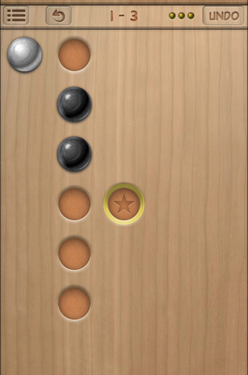
\includegraphics[scale=.5]{Initial-State-Level-3.png} \caption{Initial State}
\label{fig:Initial1}
\end{figure}

The Problem Space Model is given below:
\begin{itemize}
\item Set of States: A physical configuration of the puzzle.
\item Operators: 4 of them namely Left, Right, Up and Down.
\item Initial State: White and black balls placed at random positions with one position marked as Goal.
\item Goal State: White ball is positioned on the goal position. 
\end{itemize}


Mulled has the limitation of just being able to push a black ball but never being able to pull it back. Thus the game reaches a state which is "deadlocked" and hence it is unsolvable. The only way out is to undo a movement or to restart the game. Thus this paper tries to identify and avoid the deadlocks so that the game can be solved optimally.


\section{Related Work}
Deadlocks[1][3] have been studied for the Sokoban[2] game which is a PSPACE-complete single agent search problem. Some research has been done on the different types of deadlocks[2] in Sokoban and the techniques for avoiding them. Minimin Lookahead Search algorithm[4] has been proposed for real time problems and it might be possible to find a search horizon to detect all deadlocks in Mulled.



\section{Deadlocks}
Deadlocks are the states from which reaching the goal becomes impossible. For Mulled; states are unsolvable mainly because of the specific position of the black balls.  Once the state gets deadlocked, the game isn't solvable anymore, no matter what the user does. Thus avoiding deadlocks is of prime importance for solving the puzzle. A description of some common deadlock types is given in this section.

\subsection{Immovable Black ball on Goal Deadlock}
Immovable black ball on Goal deadlock is encountered when a black ball gets positioned on the goal position such that it is immovable in both the directions(horizontally and vertically). This deadlock is shown in Figure \ref{fig:Deadlock1} where a black ball is sitting on goal with no possibility left of pushing it horizontally or vertically.

\begin{figure}
\centering
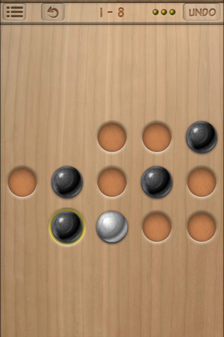
\includegraphics[scale=.5]{Deadlock-1.png} \caption{Immovable Black ball on Goal Deadlock}
\label{fig:Deadlock1}
\end{figure}

\subsubsection {Avoidance Method Algorithm}
This method will return true if the Immovable Black ball on Goal Deadlock is encountered or else it will return false.
\begin{enumerate}\addtocounter{enumi}{0}
\item Check whether a black ball is sitting on goal.
\item If No, return false.
If Yes, then check whether there is an available cell or a cell with white ball sitting on it to the left and to the right of the Goal cell.
\item If there is such a cell on both the Left and Right side of the Goal cell, return false.
\item Check whether there is an available cell or a cell with white ball sitting on it in the upward and in the downward direction with respect to the Goal cell.
\item If there is such a cell in the upward and in the downward direction with respect to the Goal cell, return false.
\item If none of the above conditions are true, return true.
\end{enumerate}
  
This method mainly checks that if there is a black ball sitting on goal; can that black ball be moved in horizontal or vertical direction so that there is a possibility of white ball positioning itself on goal cell. Before taking a move; the next state is checked against this method and the move is taken only if this method returns false. This avoids Immovable Black ball on Goal Deadlock. 

\subsection{Freeze Deadlock}
Freeze Deadlock is encountered when white ball gets placed into a cell such that no legal moves are left for it. This deadlock is shown in Figure \ref{fig:Deadlock2} where the bottom right white ball is freezed and no moves are left for it. Hence it is not possible to position this white ball on the goal cell.

\begin{figure}
\centering
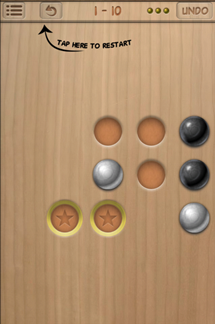
\includegraphics[scale=.5]{Deadlock-2.png} \caption{Freeze Deadlock}
\label{fig:Deadlock2}
\end{figure}

Generally this type of deadlock occurs when dealing with multiple white balls. It is not possible to encounter this deadlock with just one white ball unless the initial state is already deadlocked. As this paper only looks at the single agent search problem; the avoidance technique for this deadlock was not considered. 

\subsection{Blocked Goal Deadlock}
Blocked Goal Deadlock is encountered when all legal neighbors of goal cell are occupied by black balls such that these black balls cannot be moved in any direction except towards the goal which will create Immovable Black ball on Goal Deadlock as explained above.  Legal neighbors mean the neighbors where the cells actually exist. In Figure \ref{fig:Deadlock3} the legal neighbors of the goal cell are positioned in Right and Up direction. This deadlock is shown in Figure \ref{fig:Deadlock3} where the only legal neighbors of the goal cell are occupied by black balls and these black balls cannot be moved in any direction except towards the goal.

\begin{figure}
\centering
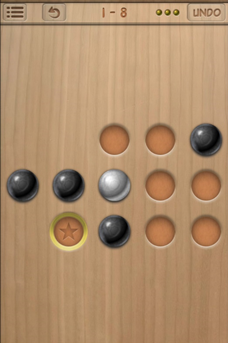
\includegraphics[scale=.5]{Deadlock-3.png} \caption{Blocked Goal Deadlock}
\label{fig:Deadlock3}
\end{figure}

\subsubsection {Avoidance Method Algorithm}
This method will return true if the Blocked Goal Deadlock is encountered or else it will return false.
\begin{enumerate}\addtocounter{enumi}{0}
\item Check whether all the legal neighbors of goal cell are occupied by black balls.
\item If No, return false.
If Yes, then run steps 3-6 for each legal neighbor of goal cell.
\item Check whether there is an available cell or a cell with white ball sitting on it to the left and to the right of this legal neighbor of goal cell.
\item If there is such a cell on both the Left and Right side of the neighbor, return false.
\item Check whether there is an available cell or a cell with white ball sitting on it in the upward and in the downward direction with respect to the legal neighbor.
\item If there is such a cell in the upward and in the downward direction with respect to the legal neighbor, return false.
\item If none of the above conditions are true, return true.
\end{enumerate}
  
This method mainly checks that if the neighbor of the goal cell has a black ball sitting on it; can that black ball be moved in horizontal or vertical direction. The intuition behind this is simple; if you need to reach the goal cell, you need to be able to reach one of the immediate neighbors of goal cell. Before taking a move; the next state is checked against this method and the move is taken only if this method returns false. This avoids Blocked Goal Deadlock. A similar strategy can be applied in order to avoid Freeze Deadlock where instead of goal cell white ball neighbors must be considered. 

  
\section{Minimin Lookahead Search}
With the help of avoidance techniques discussed; you will not encounter the deadlocks mentioned above. But there are some deadlocks which don't come under this category and it is difficult to characterize them formally. Let us consider Figure \ref{fig:Other-Deadlock} as an example. The left state in Figure \ref{fig:Other-Deadlock} is solvable but the right state is unsolvable. So if you take a move to the left from the state shown on the left you will reach the state shown on the right which is unsolvable. This means that this state is deadlocked, but this deadlock does not come under the above mentioned types and hence we would not be able to avoid this deadlock.


\begin{figure}
\centering
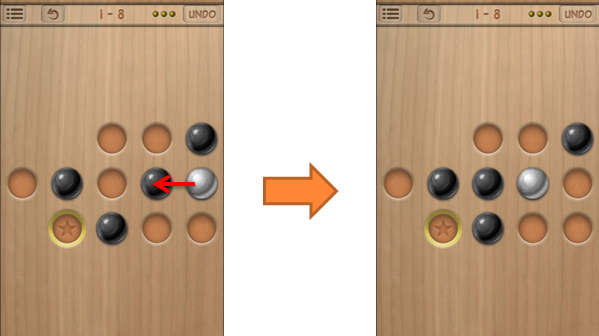
\includegraphics[scale=.5]{Other-Deadlock.png} \caption{Other Deadlocks}
\label{fig:Other-Deadlock}
\end{figure}

In order to avoid these deadlocks, the paper tries to find some minimin search horizon as searching all the way to the goal is generally not possible while playing the game in real-time. As deadlocks are generally caused because of the specific position of the black balls, the first intuition was counting the number of black balls between the current position of white ball and the goal cell along the shortest path. As there are many shortest paths between white ball and goal cell, for simplicity the paper considers only two shortest paths i.e one along the row of white ball and then moving vertically towards goal cell and the second path is to move along the row of goal cell and then moving vertically towards white ball. Based on this intuition and after trying on many initial states, a formulation for minimum search depth was calculated that is required to detect all deadlocks. If NBB denotes the number of black balls, then the formula is given as shown below:

\begin{equation}
\begin{multlined}
Minimum\;Search\;Depth \\
= \{Max(NBB\;in\;\emph{1\textsuperscript{st}}\;path , \;NBB\;in\; \emph{2\textsuperscript{nd}}\;path) + 1 \}
\end{multlined}
\label{eq:Minimin_Search_Horizon}
\end{equation}

\subsubsection{Algorithm}
Using the search horizon as given by Equation \ref{eq:Minimin_Search_Horizon}, we can avoid all deadlocks using the following algorithm:
\begin{enumerate}\addtocounter{enumi}{0}
\item Given the current state find the number of black balls positioned between the white ball and the goal cell in the two paths as discussed above.
\item Expand the search tree to a fixed depth as given by equation \ref{eq:Minimin_Search_Horizon}.
\item Evaluate the leaf nodes by \emph{f(n)} \emph{=} \emph{g(n) + h(n)} where \emph{g(n)} is the cost of reaching to the current state from the initial state and \emph{h(n)} is evaluated as the Manhattan distance between the white ball and goal cell.
\item If Blocked Goal Deadlock is encountered within the search space; backup a value of $\infty$ to the direct children of the current state that moved to this deadlocked state.
\item If Immovable Black ball on Goal Deadlock is encountered; backup a value of $\infty$ - 1 to the direct children of the current state that moved to this deadlocked state.  
\item If none of these deadlocks are encountered; backup the minimum values of all the leaf nodes to their parents.
\item Make one move to the child with the best backed value which is the one with the least \emph{f(n)} value.
\item If all the leaf nodes are deadlocked; apply the inverse operator on the current state so that it can try another path to goal. The inverse operator means taking a move in the reverse direction by applying the inverse of the operator that its parent made to reach the current state.
\item Repeat steps 1-8 until you reach the goal state or when you have tried all possible moves for all possible states.
\end{enumerate}

The Minimin Lookahead Search algorithm gives more priority to Blocked Goal deadlock as compared to Immovable Black ball on Goal Deadlock as it deals with multiple black balls as oppose to a single black ball in the other type of deadlock. The algorithm makes a locally optimal decision and tries to take a move such that it always reaches a state that is solvable. This algorithm worked perfectly well when tested against simple and normal cases that were published by the game itself. But when looked at it carefully, it was found that there are some cases that cannot avoid all deadlocks using this algorithm. For example one such case will be when the immediate neighbors don't block the Goal cell but some region ahead of the immediate neighbors is filled with black balls such that a single move will reach an unsolvable state. This type of deadlock won't be detected by the above algorithm as the goal cell is not blocked by the immediate neighbors. Thus we can see experimentally that Minimin Lookahead Search won't be able to detect all the deadlocks for all the possible cases unless we search completely till the goal.

\section{Approaches used for Solving}
The different approaches used for solving Mulled are described in short in this section.

\subsection{Approach 1: Breadth-First Search(BFS)}
The simple Breadth-First Search algorithm was used to solve the game optimally. A hashmap was used for detecting duplicate states and also the last move was stored to reduce the branching factor by 1. A queue was used for implementing BFS as the queue provides a First-in-First-out mechanism. All the 4 operators are tested against each state and all the new states are added to the queue if they are not duplicates of the previously seen states. The results of implementing BFS to solve Mulled are shown in the Results section.

\subsection{Approach 2: A*}
As a second approach, the A* algorithm was used to solve the game optimally. The manhattan distance between the white ball and the goal cell was considered as the heuristic function \emph{h(n)}. This heuristic function is admissible as the white ball will be required to take atleast the moves that are equal to the manhattan distance in order to position itself on the goal cell. Each edge was considered to have cost of 1 and hence \emph{g(n)} was simply calculated as the number of moves needed to reach the current state from the initial state. Using these definitions each node is evaluated using the following cost function:
\begin{equation}
f(n) = g(n) + h(n)
\end{equation} 
A priority queue was used for storing the nodes in the open list and also for retrieving the nodes with least \emph{f(n)} value first. A hashset was used for maintaining the closed list of already evaluated nodes. The results of implementing A* to solve Mulled are shown in the Results section.

\subsection{Approach 3: A* with Deadlock avoidance}
As the third approach, the deadlock avoidance methods discussed above were integrated with A* algorithm to check for its correctness, efficiency and time requirements. Other than this everything else was same as used in Approach 2. The results of implementing A* with Deadlock avoidance to solve Mulled are shown in the Results section.

\subsection{Approach 4: Minimin Lookahead Search}
As the final approach, the algorithm for Minimin Lookahead Search as discussed above was implemented to check whether it was possible to avoid all deadlocks using the search horizon as given by equation \ref{eq:Minimin_Search_Horizon}. It was seen that the algorithm worked well with simple and normal cases which were published by the game itself. But there were some cases where this algorithm failed and it was not possible to  avoid all deadlocks. Hence this approach failed and it was now known that in order to avoid all deadlocks in Mulled, you need to search all the way to the goal. 

\section{Results}
In order to compare the results across the 3 algorithms namely BFS, A* and A* with Deadlock avoidance; we have fixed some of the parameters of the game just for analysis. First of all the grid is assumed to be fully connected meaning every position in the grid has a valid cell. Secondly the grid is assumed to be a square with dimensions given as \emph{s*s}. Goal is fixed at the top left corner of the grid and the white ball is fixed at the bottom right corner of the grid. The number of black balls were determined empirically to make the game harder and interesting to solve which came out to be equal to 50\% of the actual number of cells in the grid. In the experiments, 100 random instances of each grid size were tested against all the three algorithms. The average result obtained after running for these 100 random instances are depicted in table \ref{Nodes and time calculated}.     
  
\begin{table*}
\Huge
\centering
\resizebox{2.25\columnwidth}{!}{%
\begin{tabular}{|c|c|c|c|c|c|c|}
\hline
Grid Size & \multicolumn{1}{|c|}{Breadth-First Search} & \multicolumn{2}{|c|}{A*} & \multicolumn{3}{|c|}{A* with Deadlock Avoidance}\\[10pt]
\hline
 & \begin{tabular}{@{}c@{}}Average \# of \\  nodes evaluated \end{tabular} & \begin{tabular}{@{}c@{}}Average \# of \\  nodes evaluated \end{tabular} & \begin{tabular}{@{}c@{}}Average time \\  taken (sec) \end{tabular} & \begin{tabular}{@{}c@{}}Average \# of \\  nodes evaluated \end{tabular} & \begin{tabular}{@{}c@{}}Average time \\  taken (sec) \end{tabular} & \begin{tabular}{@{}c@{}}Average \# of \\  deadlocks found \end{tabular} \\ 
\hline
3*3 & 3 & 3 & 0.0007467 & 1 & 0.0004740 & 1\\
\hline
4*4 & 34 & 34 & 0.0066599 & 7 & 0.0012916 & 2\\
\hline
5*5 & 1908 & 586 & 0.0300684 & 160 & 0.0173642 & 16\\
\hline
6*6 & 2106 & 633 & 0.0336428 & 473 & 0.0170462 & 31\\
\hline
7*7 & 1744 & 628 & 0.0667297 & 53 & 0.0177551 & 5\\
\hline
8*8 & 15444 & 539 & 0.0608961 & 131 & 0.0565294 & 11\\
\hline
9*9 & 64576 & 449 & 0.0641060 & 171 & 0.0327249 & 9\\
\hline
10*10 & Memory Error & 507 & 0.0417262 & 138 & 0.0046243 & 4\\
\hline
11*11 & Memory Error & 955 & 0.2731887 & 200 & 0.0117481 & 4\\
\hline
12*12 & Memory Error & 1428 & 0.7167881 & 326 & 0.0347222 & 7\\
\hline
\end{tabular}
}
\large Note : States having number of nodes evaluated greater than 100000 were ignored.\\
\large Note : States having number of deadlocks greater than 1000 were ignored.\\
\caption{Average \# of nodes evaluated in BFS, A* and A* with Deadlock Avoidance, average time taken in A* and A* with Deadlock Avoidance and average number of deadlocks found in A* with Deadlock Avoidance}
\label{Nodes and time calculated}
 
\end{table*}

Table \ref{Nodes and time calculated} gives the average number of nodes evaluated and average time taken for the respective algorithms and the average number of deadlocks found for A* with deadlock avoidance algorithm. For all the experiments, states having number of nodes evaluated greater than 100000 were ignored as memory was a limiting issue while running the program. Even the States having number of deadlocks greater than 1000 were ignored because memory was a problem and also because these were generally the unsolvable states that were encountering more deadlocks than actual useful states.

Table \ref{Nodes and time calculated} shows us that the average number of nodes evaluated and the average time taken by A* with deadlock avoidance algorithm is lower as compared to both A* and BFS. A* evaluated less number of nodes as compared to BFS which is a well known fact. BFS failed to give output when grid size became 10 and more. The column of deadlocks gives the average number of  times the Immovable Black ball on Goal Deadlock or the Blocked Goal Deadlock were encountered by the states of that particular grid size.

The experimental results prove that A* with deadlock avoidance is the best algorithm for solving Mulled both in terms of nodes evaluated and the time taken for running the algorithm. This algorithm is complete as the minimum positive edge cost is 1 and the heuristic values are never negative as it is the manhattan distance between the white ball and goal cell. The algorithm gives optimal results as the manhattan distance heuristic never overestimates the actual cost to the goal. The time and space requirements for this algorithm are same as that of A*. Thus by implementing simple methods that avoid deadlocks we are able to reduce the number of evaluated nodes and time significantly. This reduction is mainly due to the time saved by not evaluating the deadlocked states themselves and also their children.   


\section{Conclusions}
The characterization and avoidance of deadlocks helps significantly in reducing the time and the number of nodes needed to be evaluated in order to solve any puzzle in general. A* with deadlock avoidance algorithm was found to be the best algorithm for solving Mulled. The concept of Minimin Lookahead Search was found to be not applicable to Mulled for finding all deadlocks. For detecting all the deadlocks, you need to search all the way to the goal.

\section{Future Scope}
Firstly as seen it was difficult to characterize all the deadlocks present in Mulled. So one can try to characterize these deadlocks which will make Mulled almost deadlock free. Also one could try solving states having multiple white balls instead of just a single white ball as considered in this paper. As memory is the limiting factor for A* in general, it would be worth trying out other memory efficient algorithms like frontier search, depth-first branch and bound etc for solving Mulled. 

\section{References}

[1] Cazenave, Tristan, and Nicolas Jouandeau. "Towards
deadlock free Sokoban." (2010). \newline
[2] http://sokobano.de/wiki \newline
[3] Junghanns, Andreas, and Jonathan Schaeffer.
"Sokoban: Evaluating standard single-agent search
techniques in the presence of deadlock." Advances in
Artificial Intelligence. Springer Berlin Heidelberg, 1998.
1-15.\newline
[4] Korf, Richard E. "Real-Time Heuristic Search: First
Results." AAAI. 1987.\newline
[5] Korf, Richard E. "Heuristic Search"\newline
[6] http://hakogames.com/\newline
[7] https://play.google.com/store/apps\newline
/details?id=com.HakoGames.MulledAndroidFreewline\newline

\end{document}
